%=========================================
% 	   Fallbeispiel     		 =
%=========================================
\chapter{Fallbeispiel}

\section{Beschreibung}
\section{Anforderungen}

\begin{figure}[bth] 
	\centering
	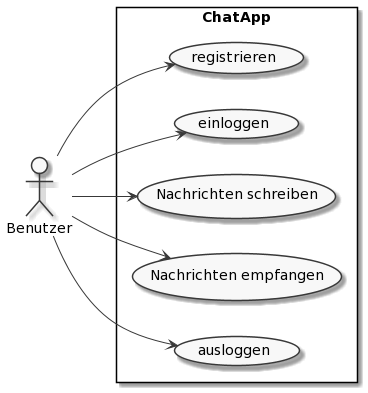
\includegraphics[width=0.6\textwidth]{Graphics/Usecase-Diagramm.png}
	\caption{Use-Case Diagramm}
\end{figure}

\section{Architekturentwurf}

\begin{figure}[bth] 
	\centering
	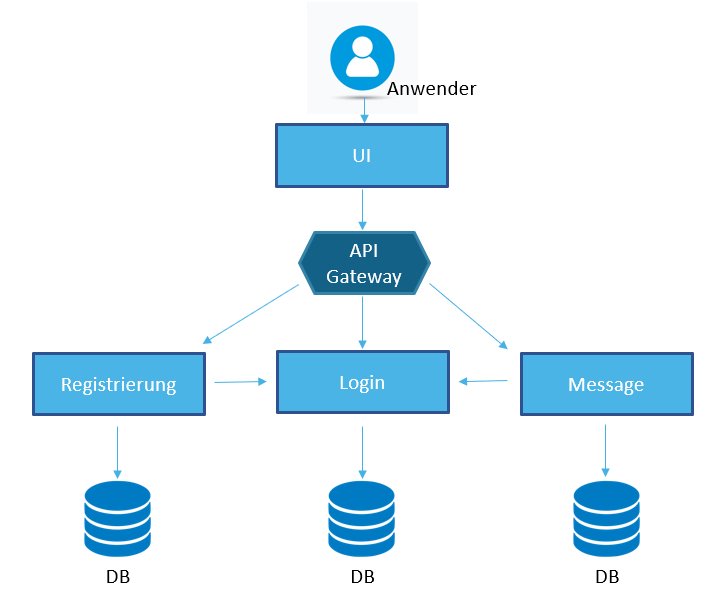
\includegraphics[width=0.6\textwidth]{Graphics/Architekturentwurf.png}
	\caption{Architekturentwurf}
\end{figure}

\begin{figure}[bth] 
	\centering
	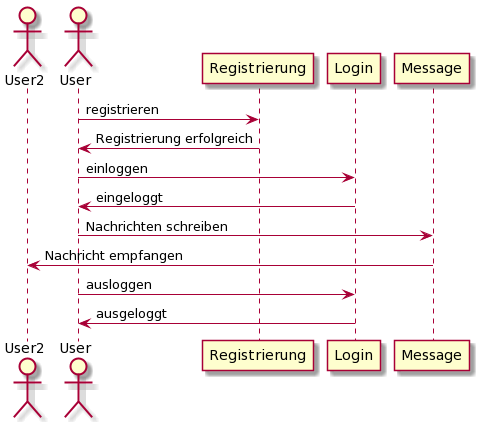
\includegraphics[width=0.6\textwidth]{Graphics/Sequenzdiagramm.png}
	\caption{Sequenzdiagramm}
\end{figure}

\section{Implementierung des Prototyps}
auch genutzte Technologien aufzeigen

